\documentclass[letterpaper,10pt,onecolumn]{article}
\usepackage[spanish]{babel}
\usepackage[utf8x]{inputenc}
\usepackage{amsfonts}
\usepackage{amsthm}
\usepackage{amsmath}
\usepackage{mathrsfs}
\usepackage{empheq}
\usepackage{enumitem}
\usepackage[pdftex]{color,graphicx}
\usepackage{hyperref}
\usepackage{listings}
\usepackage{calligra}
\usepackage{algpseudocode} 
\DeclareMathAlphabet{\mathcalligra}{T1}{calligra}{m}{n}
\DeclareFontShape{T1}{calligra}{m}{n}{<->s*[2.2]callig15}{}
\newcommand{\scripty}[1]{\ensuremath{\mathcalligra{#1}}}
\lstloadlanguages{[5.2]Mathematica}
\setlength{\oddsidemargin}{0cm}
\setlength{\textwidth}{490pt}
\setlength{\topmargin}{-40pt}
\addtolength{\hoffset}{-0.3cm}
\addtolength{\textheight}{4cm}

\begin{document}
\begin{center}



\includegraphics[width=490pt]{header.png}\\[0.5cm]

\textsc{\LARGE Taller 10 - F\'isica I (FISI-1018) - 2016-10}\\[0.5cm]

\textsc{\Large{Profesor: Jaime Forero}} \\[0.5cm]

\noindent\textsc{Ejercicios correspondiente a la clase complementaria de la semana del 4 de abril del 2016.}\\[0.5cm]
\end{center}

\noindent\textsc{Nota:} 
Los primeros tres ejercicios deben ser
entregados {\bf al comienzo} de la clase complementaria. Los \'ultimos
seis deben ser trabajados {\bf durante} la complementaria. 

La numeraci\'on
hace referencia al texto gu\'ia: \textit{F\'isica Universitaria Volumen
  1 (Sears-Semansky)}, decimotercera edici\'on, Pearson.

\begin{enumerate}

% aqui vienen los tres ejercicios "faciles"
\item Ejercicio 9.2 H\'elice de un avi\'on.
\item Ejercicio 9.10 Ventilador que se apaga.
\item Ejercicio 9.18 Contrapeso de un elevador antiguo.
\item Calcule el momento de cada uno de los siguientes objetos. 
 \begin{enumerate}
\item Una bola de $0.5kg$ lanzada hacia arriba con velocidad de $30m/s$. 
\item Un auto de $2000kg$ que se mueve a $10m/s$ hacia el sur.
\item Un electrón de masa de $9.1×10^{–31}kg$, moviéndose a una velocidad de $1.0×10^7m/s$.
\item  La tierra, de masa $6.0×10^{24}kg$, Moviéndose alrededor de su orbita con velocidad de $3.0×10^4m/s$.
\end{enumerate}
%Miguel
% aqui vienen los cuatro ejercicios "dificiles"
\item Un automóvil de $1500kg$. De masa choca contra un muro. La velocidad inicial del automóvil es $\vec{V}_i=-15m/s\hat{i}$, la velocidad final del móvil es $\vec{V}_f=2.6m/s\hat{i}$. Si el choque dura $0.15s$, encuentre el impulso y la fuerza promedio ejercida sobre el automóvil?
%Miguel
\item Una bala de masa $m=250g$ choca contra un bloque de $M=3.8kg$ suspendido de una cuerda de $L=80cm$ de larga y en reposo. Después del choque el sistema bloque$-$bala forma un ángulo de $\theta=30^{\circ}$ con la vertical. Calcular:
\begin{enumerate}
\item La velocidad del saco y la bala inmediatamente después del choque.
\item  La velocidad $v_0$ de la bala antes del choque. 
\begin{figure}[h]
\begin{center} 
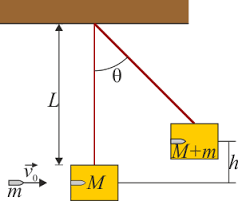
\includegraphics[scale=0.5]{bloquebalistico.png} 
\end{center} 
\end{figure}
\end{enumerate}
%Miguel
\item Una bola de masa $m$ está atada a un punto fijo por medio de una cuerda de longitud $L$. Un viento muy fuerte ejerce sobre la bola una fuerza constante, de magnitud $F$, de izquierda a derecha, como se muestra en la figura.
\begin{center} 
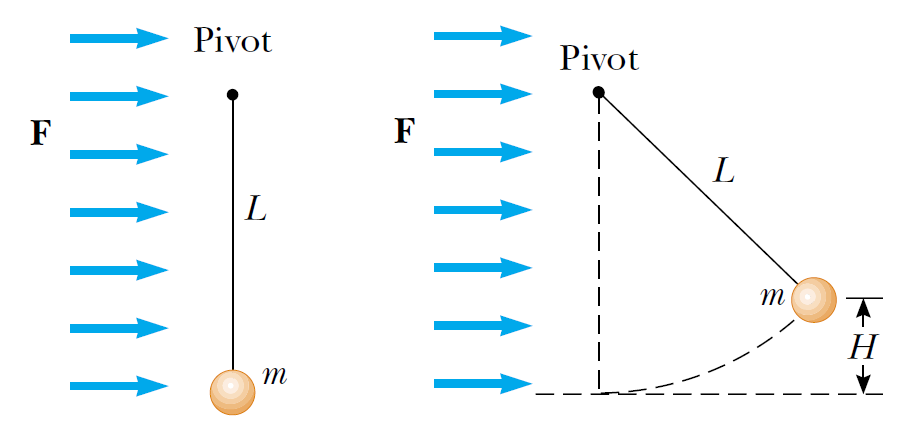
\includegraphics[scale=0.5]{bolaviento} 
\end{center} 
\begin{enumerate}
\item Si la bola estaba inicialmente en reposo, muestre que la altura máxima que alcanza la bola está dada por la expresión:
\begin{align}
H_{max}=\frac{2L}{1+(mg/F)^2}
\end{align}
\item Halle una expresión para la altura de equilibrio de la bola en presencia de la fuerza $F$
\end{enumerate} %Juan Carlos
\item Una persona de 45 kg se encuentra sobre un planchón de 150 kg que a su vez está sobre un lago congelado, sobre dicha superficie el planchón puede deslizar sin fricción. La persona camina sobre el planchón con una velocidad constante de 1.5 m/s.
\begin{enumerate}
\item ¿Cuál es la velocidad de la persona con respecto a la superficie del lago?
\item ¿Cuál es la velocidad del planchón con respecto a la superficie del lago?
\end{enumerate} %Juan Carlos
\item Una bola de plastilina de 12g es arrojada horizontalmente contra un bloque de madera de 100 g que se encuentra en reposo. La plastilina queda totalmente pegada al bloque de madera y el sistema se mueve 7.5 m con respecto a la posición inicial del bloque de madera. Si el coeficiente de fricción entre el bloque de madera y la superficie sobre la que se desliza es de 0.65, ¿cuál era la velocidad de la bola de plastilina justo antes de impactar al bloque de madera? %Juan Carlos

\end{enumerate}
 

\end{document}


\begin{figure}[h]
\begin{center} 
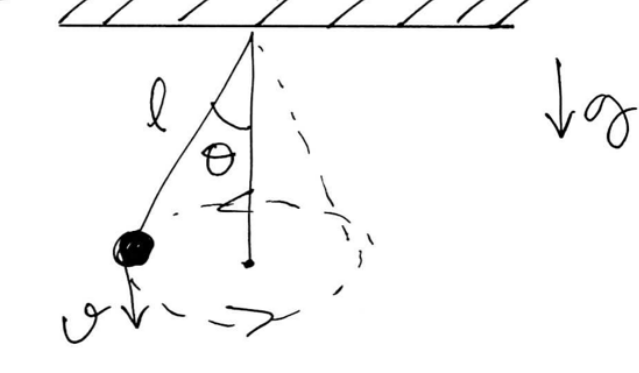
\includegraphics[scale=0.25]{conico.png} 
\caption{\label{fig:conico}Figure para el problema \ref{conico}}
\end{center} 
\end{figure}

\begin{figure}[!h]
\begin{center}
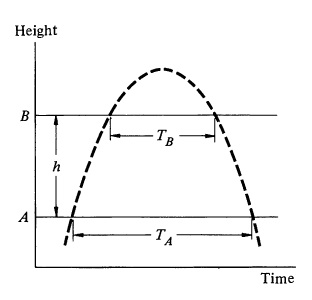
\includegraphics[scale=0.7]{altura.jpg} 
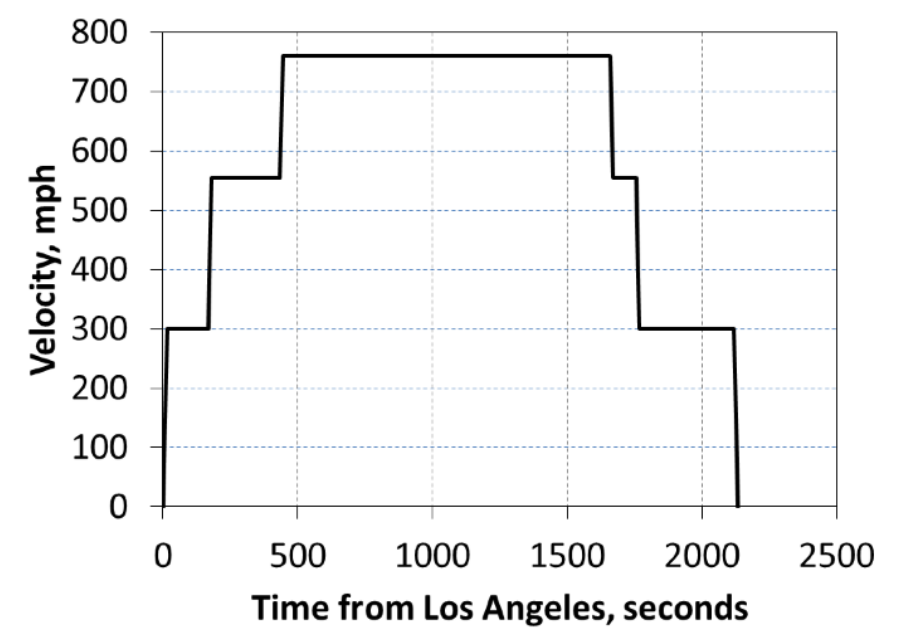
\includegraphics[scale=0.3]{hyperloop.png} 
\end{center}
\caption{Izquierda: diagrama para el ejercicio recomendado 3. Derecha: diagrama para el ejercicio recomendado 4.}
\label{fig:tiro}
\end{figure}





